
\chapter{ANALYSIS}
\label{ch:Analysis}

\section{Security}

Now we examine and compare OnioNS' central protocols against our security assumptions and expected threat model.

% Tor circuits work, no global attacker, privacy and anonymity achieved, no crypto breaks
% Tor isn't entirely honest, but the majority is honest
% Eve cannot break Tor in response to OnioNS, Eve cannot guess quorum
% The largest set of agreeing nodes in the Quorum is honest

\subsection{Quorum Selection}

The Quorum nodes have greater attack capabilities than any other class of participants in OnioNS. In our threat model, we assume that an attacker, Eve, already has control of some fixed number $ f_{E} $ of routers in the Tor network, and that her nodes may maliciously collude. It is also impossible to determine which Tor routers are under Eve's control and which are honest in advance, so we examine our Quorum protocols and explore the likelihood of attacks within a probabilistic environment.

The Quorum Derivation protocol selects an $ L_{Q} $-sized subset of routers from the set of Quorum Candidates, and rotates this selection every $ \Delta q $ days. The optimal selection of $ L_{Q} $ and $ \Delta q $ is dependent on both security and performance analysis; our security analysis introduces a lower bound on both $ L_{Q} $ and $ \Delta q $. For the following evaluations, we feel it safe to discard threats that have probabilities at or below $ \frac{1}{2^{128}} \approx 10^{-38.532} $ --- the probability of Eve randomly guessing a 128-bit AES key, a threat that would violate our security assumption on the security of Tor circuits.

We assume that $ L_{Q} $ will be selected from a pool of 5,400 Quorum Candidates --- the number, as of April 2015, of Tor routers with the Fast and Stable flags, whom we assume are all up-to-date Mirrors. Let $ L_{E} $ be the number of Quorum nodes under Eve's control. Then Eve controls the Quorum if the $ L_{E} $ routers become the largest agreeing subset in the Quorum, which can occur if either more than $ \frac{L_{Q} - L_{E}}{2} $ honest Quorum nodes disagree or if $ L_{E} > \frac{L_{Q}}{2} $. The second scenario can be statistically modelled.

Quorum selection is mathematically an $ L_{Q} $-sized random sample taken from an $ N $-sized population without replacement, where the population contains a subset of $ f_{E} $ entities that are considered special. Then the probability that Eve controls $ k $ Tor routers in the Quorum is given by the hypergeometric distribution, whose probability mass function (PMF) is $ \frac{\binom{f_{E}}{k}\binom{N - f_{E}}{L_{Q} - k}}{\binom{N}{L_{Q}}} $. Then the probability that $ L_{E} > \frac{L_{Q}}{2} $ is given by $ \displaystyle\sum_{x=\ceil{\frac{L_{Q}}{2}}}^{L_{Q}} \frac{\binom{f_{E}}{k}\binom{N - f_{E}}{L_{Q} - k}}{\binom{N}{L_{Q}}} $. Odd choices for $ L_{Q} $ prevents the possibility of network disruption when the Quorum is evenly split in terms of the current Page. We examine the probability of Eve's success for increasing amounts of $ f_{E} $ in Figure \ref{chart:quorumMajority}.

\begin{figure}[htbp]
	\centering
	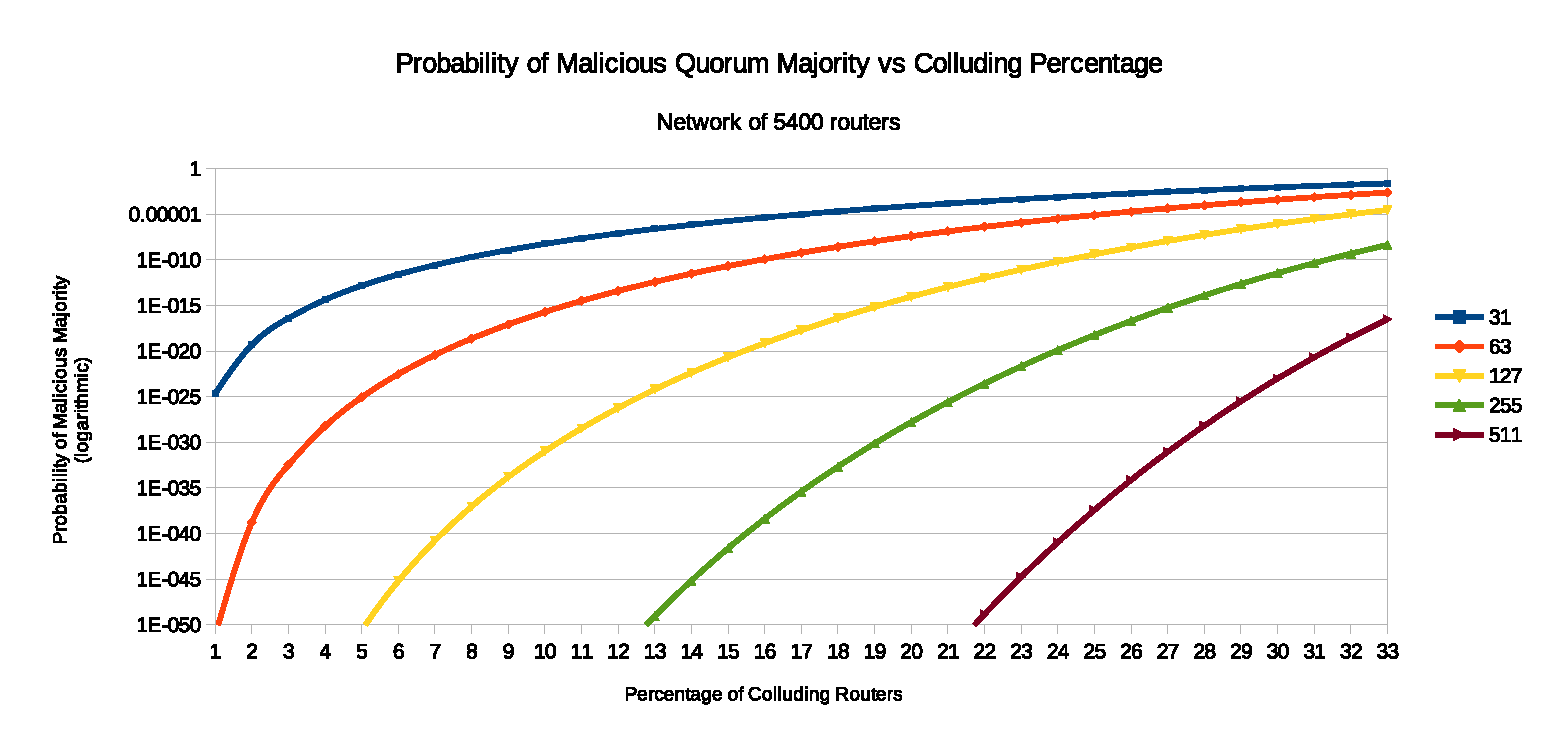
\includegraphics[width=1\textwidth]{analysis/MaliciousQuorumProbability.eps}
	\caption{The probability that Eve controls the majority of the Quorum is given by the PMF of the hypergeometric distribution. We fix $ N $ at 5,400 nodes and graph Eve's success probability as a function of an increasing percentage of Eve-controlled colluding routers. We examine five selections for $ L_{Q} $: 31, 63, 127, 255, and 511. We do not consider percentages beyond 33 percent as those represent a near-complete compromise of the Tor network.}
	\label{chart:quorumMajority}
\end{figure}

Figure \ref{chart:quorumMajority} shows that a choice of $ L_{Q} = 31 $ is suboptimal: the probabilities are above the $ 10^{-38.532} $ threshold for even small levels of collusion. $ L_{Q} = 63 $ likewise fails with approximately two percent collusion, although choices of 127, 255, and 511 fail at levels above approximately 8, 16, and 25 percent, respectively. The figure also suggests that larger Quorums are superior with respect to security. Small Quorums are also less resilient to DDOS attacks at the Quorum in general.

If we assume that Eve controls 10 percent of the Tor network, then we can examine the impact of the longevities of Quorums; over a fixed period of time, slower rotations suggests a lower cumulative chance of selecting any malicious Quorum. If $ w $ is Eve's chance of compromise, then her cumulative chances of compromising any Quorum is given by $ 1 - (1-2)^t $. This gives us a bound estimate on $ \Delta q $. We estimate this over 10 years in Figure \ref{chart:cumulativeProbability}.

\begin{figure}[htbp]
	\centering
	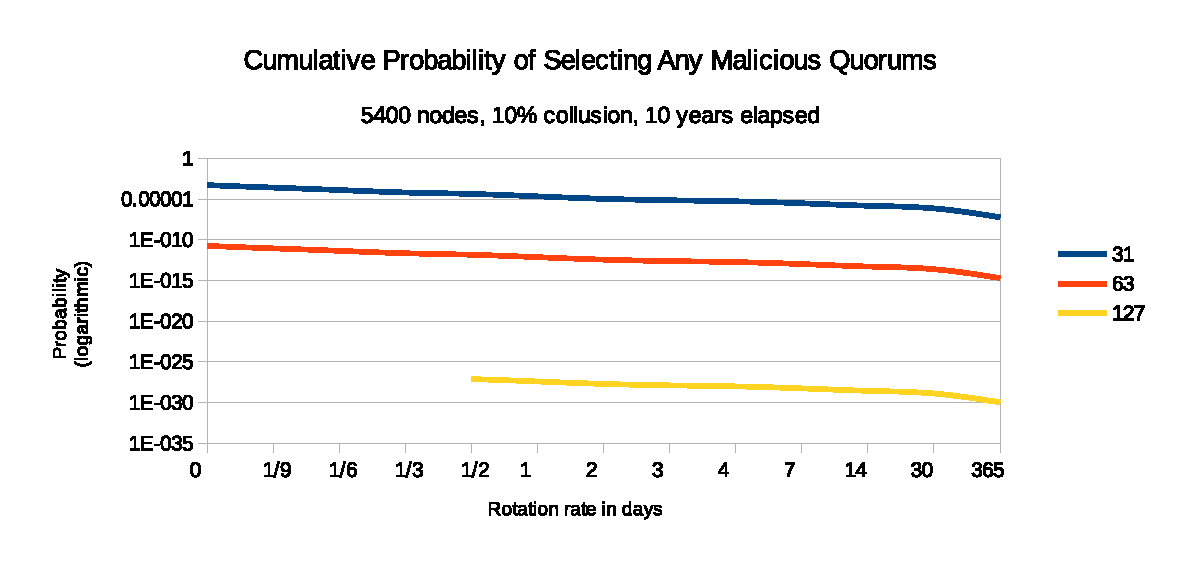
\includegraphics[width=1\textwidth]{analysis/CumulativeMaliciousQuorum.eps}
	\caption{The cumulative probability that Eve controls any Quorum at different rotation rates. We assume 10 percent collusion in a network of 5400 Tor routers, and view across 10 years. We do not graph $ L_{Q} $ values of 255 or 511 as they generate probabilities far below our $ 10^{-38.532} $ threshold; $ L_{Q} = 255 $ and $ L_{Q} = 511 $ produce values less than $ 10^{-58} $ and $ 10^{-134} $, respectively.}
	\label{chart:cumulativeProbability}
\end{figure}

Figure \ref{chart:cumulativeProbability} suggests that while slow rotations (i.e a period of 7 days) generates orders of magnitude less chance than fast rotations, the choice of $ L_{Q} $ is far more significant. Like Figure \ref{chart:quorumMajority}, it also shows that $ L_{Q} = 31 $ and $ L_{Q} = 61 $ are relatively poor choices.

If a selected Quorum is malicious, fast rotation rates will minimize the duration of any disruptions, a contradiction to Figure \ref{chart:quorumMajority}. However, given the very low statistical likelihood of selecting a malicious Quorum, we consider this a minor contribution to the decision.

Although a malicious Quorum would have the capabilities to deploy a variety of attacks on the network, the proper selections of $ L_{Q} \geq 127 $ and $ \Delta q \geq 1 $ reduces the likelihood of this occurring to near-zero probabilities. We consider this a stronger solution than introducing countermeasures to those attacks. However, the networking and performance load scales linearly with Quorum size. Based on this balance and our above analysis, we suggest 127 or 255 for values of $ L_{Q} $ and 7 or 14 for $ \Delta q $.

\subsection{Entropy of Tor Consensus Documents}
\label{sec:docEntropy}

We use Tor's consensus documents as a sources of entropy agreed upon by all parties, however we have not yet demonstrated that the network status contains enough entropy to provide reasonable assurance that Eve cannot guess the next Quorum in advance. If Eve could predict future Quorums, Eve can subvert the Quorum Derivation protocol in a variety of attack vectors. However, this would fail our security assumption against adaptive compromise in the presence of OnioNS. Rather than introducing defences against these attack vectors, we nevertheless believe that ensuring sufficient entropy in the consensus documents is a superior defence.

Periodically, Tor routers upload signed \emph{descriptors} --- routing information, cryptographic keys, and other information --- to Tor's directory authorities (dirauths). Once per hour, the dirauths aggregate and republish the descriptors back to the network, enabling Tor's network to be dynamic and distributing new information to all parties in an efficient and timely manner. While Tor provides no guarantee that the network is using the same consensus at the same time, the consensus is timestamped, so we can reference it by their time of publication. We focus on two essential documents that clients assemble from the consensus: \emph{cached-certs}, a list of long-term identity and short-term signing RSA keys from each dirauth; and \emph{cached-microdesc-consensus}, essential information about each router, such as networking information and capabilities. Since the dirauths publish a new consensus every hour, we must analyse the entropy rate between consecutive hours.

We constructed a first-order Markov model and estimated the entropy of the \emph{cached-microdesc-consensus} document by analysing the transitions for various fields between consecutive consensuses. We also provide analysis on the dynamics of the Tor network by counting routers that enter or leave the Tor network between consecutive consensuses in Figure \ref{fig:xorRouters}. Here we identity routers by their identity keys; just as Tor does, we consider routers that change their identity keys as two different routers; one leaving and one entering the network. Routers entering the network introduce significant amounts of information into the consensus. For example, \emph{cached-microdesc-consensus} contains the 160-bit SHA-1 hash of the router's RSA-1024 identity key, which are generated through OpenSSL. Thus new routers contribute at least 160 bits of information. Figure \ref{fig:xorRouters} suggests that we may expect approximately 100 to 175 routers to leave or enter the network per hour. Thus we may expect approximately 16,000 to 28,000 bits of entropy per hour from this dynamic.

\begin{figure}[h]
	\centering
	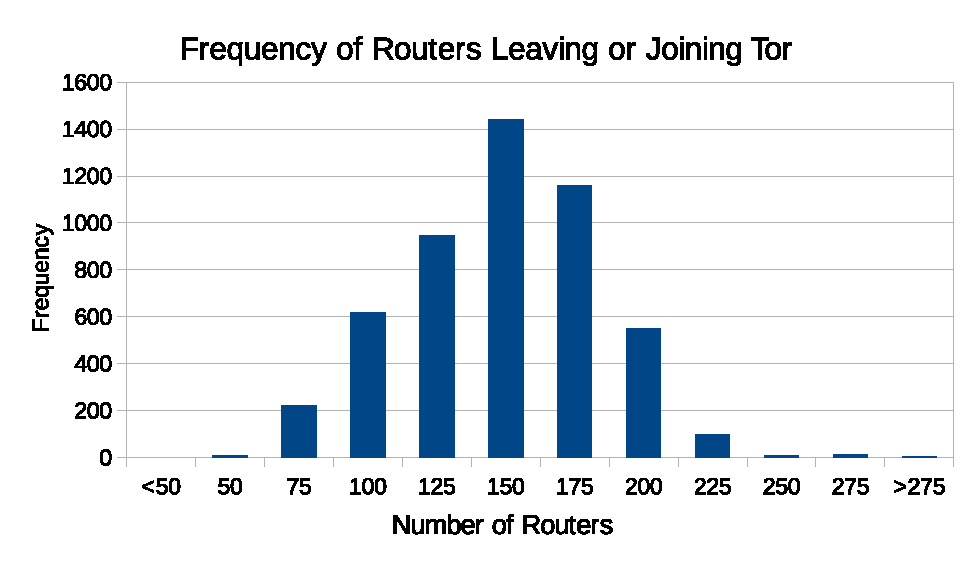
\includegraphics[width=0.7\linewidth]{analysis/LeaveJoinFrequency.eps}
	\caption{A histogram of the number of routers entering or leaving the network between consecutive consensuses across the seven-month period.}
	\label{fig:xorRouters}
\end{figure}

For routers that are present between consecutive pairs, we focus on six critical fields from each router's descriptor inside \emph{cached-microdesc-consensus}: \emph{nickname}, the router's name chosen by its operator or a default name; \emph{publication}, the time when it last published a descriptor; \emph{IP address}, its network address; \emph{ORPort}, the network port for onion routing; \emph{version}, the version of the Tor protocol that this relay is running; and \emph{bandwidth}, as self-reported or as measured by the dirauths. Tor routers change \emph{publication} when either 18 hours has elapsed since the last descriptor publication, its fields have changed, or if its uptime has been reset.

We obtained from \url{collector.torproject.org} 5,067 archived hourly publications of \emph{cached-microdesc-consensus} across a seven-month period between September 1, 2014 00:00 UTC and March 31, 2015 23:00 UTC. We construct a Markov model for the six aforementioned fields and illustrate the number of observed transitions for each field in Figure \ref{fig:transitionCount}.

\begin{figure}
	\centering
	\begin{minipage}[t]{.47\textwidth}
  		\centering
  		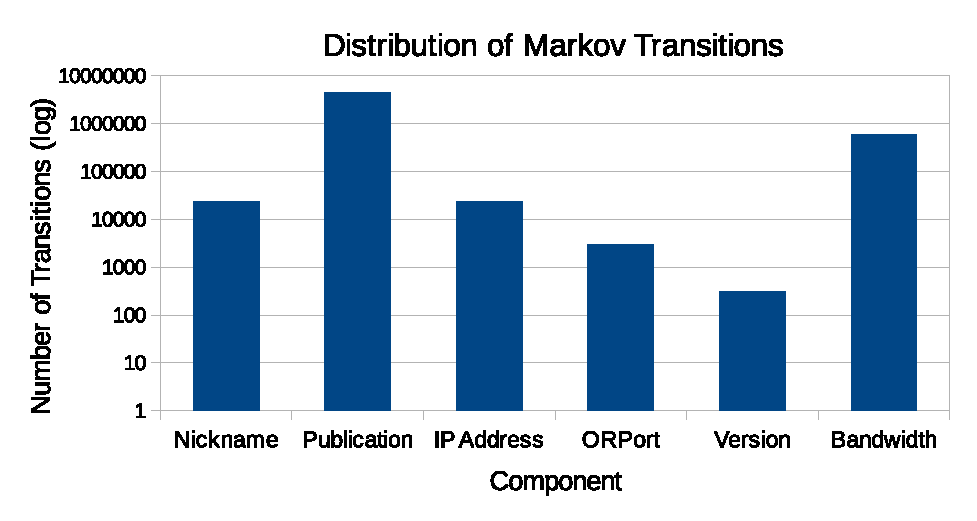
\includegraphics[width=\linewidth]{analysis/MarkovTransitionDistribution.eps}
  		\captionof{figure}{The number of observed transitions for \emph{nickname}, \emph{publication}, \emph{IP address}, \emph{ORPort}, \emph{version}, and \emph{bandwidth} between consecutive consensuses across the seven-month period.}
  		\label{fig:transitionCount}
	\end{minipage}%
	\hspace{0.7cm}
	\begin{minipage}[t]{.47\textwidth}
		\centering
		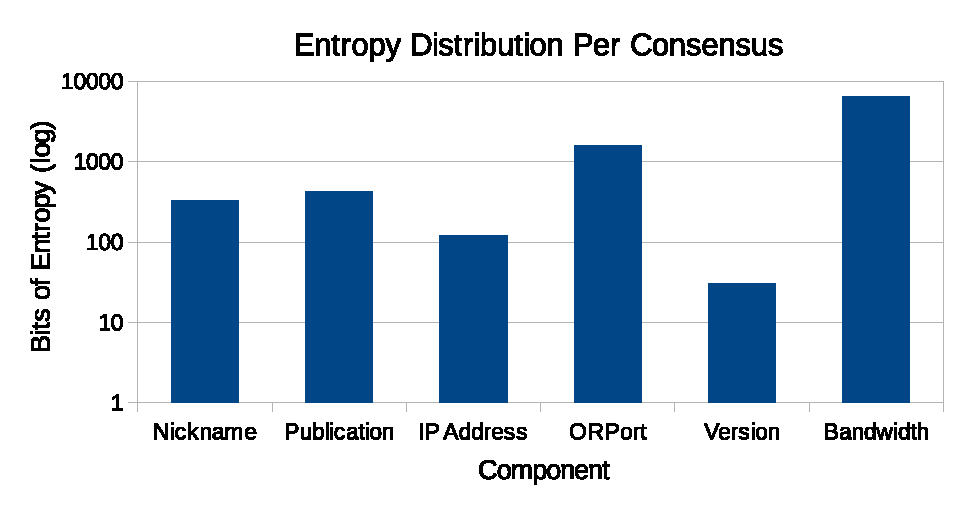
\includegraphics[width=\linewidth]{analysis/EntropyDistribution.eps}
		\captionof{figure}{The entropy rate distribution for each of the six fields in \emph{cached-microdesc-consensus}, scaled by the average size of the Tor network.}
		\label{fig:entropyRates}
	\end{minipage}
\end{figure}

Then the entropy rate is given by equation \ref{eq:entropyRate}, where $ P_{i} $ is the probability of state $ i $ and $ P_{i}(j) $ is the probability of state $ j $ given $ i $ (the $ i $-$ j $ transition). We multiply the entropy rate by the total number of routers in the Tor network. This assumes that router's are independently and uniformly distributed, but this is not always the case as small sets of routers may be managed together and change as one. However, identifying these sets and analysing them separately is non-trivial to impossible; administrators may operate anonymously or try to purposely hide their management of multiple geographically-distance routers. Due to this, this assumption results in an estimation of the entropy and not an exact value. We calculate this rate estimation for each of the six fields and illustrate the results in Figure \ref{fig:entropyRates}.

\begin{equation}
\mathrm{H}(\mathcal{S}) = - L_{T} \sum_{i} P_{i} \sum_{j} P_{i}(j) \log_{2}P_{i}(j)
\label{eq:entropyRate}
\end{equation}

The average size of the Tor network across the seven-month period was 6,672 routers, thus together these fields contributed on average approximately 8,896.7 bits of entropy per hour across our seven-month view. The two documents contain at least this much entropy; our analysis does not comprehensively cover all the fields in \emph{cached-certs} and \emph{cached-microdesc-consensus}, so other fields may also contribute additional information. Based on this analysis, the approximately 16,000 to 28,000 entropy bits contributed hourly by routers joining or entering the Tor network, and our previous statistical calculations, we conclude that with $ L_{Q} \geq 127 $, the Quorum Formation protocol is secure under our design assumptions. Our analysis shows that the size and dynamic nature of the Tor network provides the strongest defence against Quorum-level attacks.

\subsubsection{Malicious Entropy Reduction}

The Quorum Derivation protocol describes initializing the Mersenne Twister with a 384-bit seed. If we assume that Eve desires that the Quorum Derivation protocol produce a Quorum pleasing to Eve (such as including her malicious routers in the Quorum or rejecting specific honest routers from the Quorum) based on some hash $ k $. As $ H(x) $ is SHA-384, SHA-384's strong resistance to preimage attack forces Eve to spend $ L_{T} * 2^{383} $ operations on average to find $ k $. Eve may also try to manipulate her router's descriptors such that $ H(\mathit{cd}_{q+1}) = k $, but SHA-384's resistance to second-preimage attacks also requires this to require $ L_{T} * 2^{383} $ operations as well. The number of operations involved in this attack vector is significantly more than the operations involved in breaking AES, so we disregard the possibility of manipulating the Quorum Derivation protocol in this way.

\subsection{Sybil Attacks}

Eve may also attempt to increase her probability of including her malicious nodes in the Quorum via Sybil attacks. We offer no defence against this type of attack, although Tor does. The attack is difficult to carry out in practice due to the slow build of trust within the Tor network. Directory authorities would give Eve's nodes the Fast and Stable flags after weeks of continual uptime and a history of reliability. For large-scale Sybil attacks, this introduces a significant time and financial cost to Eve. We also note that choices of $ L_{Q} $ and $ \Delta q $ also offer significant statistical defences against Sybil attacks, as illustrated in Figures  \ref{chart:quorumMajority} and \ref{chart:cumulativeProbability}, shown above.

\subsection{Hidden Service Spoofing}

OnioNS does not require a hidden service operator to reveal any personally-identifiable information. Hidden services are only known by their public key and domain names, and we assume that the hidden service is authentic. We have also observed spoofed hidden services in the wild, suggesting that this problem already exists in Tor's environment. We do not introduce a reputation system or distributed verification system, and note that it is difficult if not impossible to construct a reliable defence against hidden service spoofing attacks due to their anonymous nature. 

One possible solution, although it severely compromises anonymity, is to register a hidden service with an SSL Certificate Authority and apply an SSL certificate to the server. In this way, TLS communication provides an authenticity check against the hidden service, although TLS also sets up a redundant encryption layer that may decrease performance. However, in practice this solution is very rarely seen; out of approximately 25,000 hidden services\cite{TorMetrics}\cite{kadianakis2015extrapolating}, to date only three hidden services have browser-trusted SSL certificates: Blockchain.info at https://blockchainbdgpzk.onion, Facebook at https://facebookcorewwwi.onion, and The Intercept's SecureDrop instance at https://y6xjgkgwj47us5ca.onion. In future work we may study the security implications of signing the .onion address or the .tor OnioNS domain name. Due to their severe privacy concerns and the security controversy surrounding the centralized CA Chain of Trust, generally speaking we do not recommend the application of SSL certificates to Tor hidden services. 

\subsection{Outsourcing Record Proof-of-Work}

%Scrypt introduces a cost and its memory demands increases the difficulty of custom hardware and massively-parallel attacks, effectively limiting adversaries to the same hardware as legitimate users.

The Record Generation protocol can safely take place within an offline machine under the operator's control. We designed the Record Generation protocol with the objective of requiring the hidden service operator to also perform the scrypt proof-of-work. However, our protocol does not entirely prevent the operator from outsourcing the computation to secondary resource in all cases.

Let Bob be the hidden service operator, and let Craig be a secondary computational resource. We assume that Craig does not have Bob's private key. Then,

\begin{enumerate}
	\item Bob creates an initial Record $ R $ and completes the \emph{type}, \emph{name}, \emph{nameList}, \emph{contact}, and \emph{consensusHash} fields.
	\item Bob sends $ R $ to Craig. Let $ \mathit{central} $ be $\mathit{type} \concat \mathit{name} \concat \mathit{nameList} \concat \mathit{contact} \concat \mathit{consensusHash} \concat \mathit{nonce} $.
	\item Craig generates a random integer $ K $ and then for each iteration $ j $ from 0 to $ K $,
		\begin{enumerate}
			\item Craig increments \emph{nonce}.
			\item Craig sets \emph{PoW} as $ \mathrm{PoW}(\mathit{central}) $.
			\item Craig saves the new $ R $ as $ C_{j} $.
		\end{enumerate}
	\item Craig sends all $ C_{0 \le j \le K} $ to Bob.
	\item For each Record $ C_{0 \le j \le K} $ Bob computes
		\begin{enumerate}
			\item Bob sets \emph{pubHSKey} to his public RSA key.
			\item Bob sets \emph{recordSig} to $ S_{\mathit{RSA}}(m, r) $ where $ m = \mathit{central} \concat \mathit{pow} $ and $ r $ is Bob's private RSA key.
			\item Bob has found a valid record if $ H(\mathit{central} \concat \mathit{pow} \concat \mathit{recordSig}) \leq 2^{\mathit{difficulty}} $
		\end{enumerate}
\end{enumerate}

% todo: calculate chances of Craig computing a correct record

Our protocol ensures that Craig must always compute more scrypt iterations than necessary; Craig cannot generate \emph{recordSig} and thus cannot compute if the hash is below the threshold. Moreover, the scrypt work incurs a cost onto Craig that must be compensated financially by Bob. Thus the Record Generation protocol places a lower bound on the cost paid by Bob.

%\subsection{False Negatives Claims}
%
%OnionNS records are self-signed and include the hidden service's public key, so anyone --- particularly the client --- can confirm the authenticity (relative to the authenticity of the public key) and integrity of any record. This does not entirely prevent Sybil attacks, but this is a very hard problem to address in a distributed environment without the confirmation from a central authority. However, the proof-of-work component makes record spoofing a costly endeavour, but it is not impossible to a well-resourced attacker with sufficient access to high-end general-purpose hardware.
%
%Hidden service .onion addresses will continue to have an extremely high chance of being securely unique as long the key-space is sufficiently large to avoid hash collisions.
%
%As we have stated earlier, falsely claiming a negative on the existence of a record is a problem overlooked in other domain name systems. One of the primary challenges with this approach is that the space of possible names so vast that attempting to enumerate and digitally sign all names that are not taken is highly impractical. Without a solution, this weakness can degenerate into a denial-of-service attack if the DNS resolver is malicious towards the client. Our counter-measure is the highly compact hashtable bitset with a Merkle tree for collisions. We set the size of the hashtable such that the number of collisions is statistically very small, allowing an efficient lookup in $ \mathcal{O}(1) $ time on average with minimal data transferred to the client.

\subsection{DNS Leakage}

Human mistakes can also compromise user privacy. One such security threat is the accidental leakage of .tor lookups over the Internet DNS. This vulnerability is not limited to OnioNS and applies to any alternative DNS; users may mistakenly attempt lookups over the traditional Internet DNS. Mohaisen and Thomas observed .onion lookups on root DNS servers at a frequency that corresponded to external global events, highlighting the human factor in those leakages\cite{thomasmeasuring}. For OnioNS, this may occur if their client software was not properly configured, if their browser was not properly configured to or could not communicate with Tor, or for other reasons. We offer no defence against this attack vector and note that any defence against it would need to introduce lookup whitelists or blacklists into common browsers such as Chrome, Firefox, and Internet Explorer to prevent them from attempting lookups for pseudo-TLDs.

%\section{Reliability}

%\subsubsection{Flooding}

%\emph{What happens if Quorum nodes are unavailable? How is their unavailability secured for future reference? What are the implications of a Quorum node withholding or forging a Record before flooding their Snapshot out? Can a single node mislead the rest of the Quorum?}

%Although this approach does not entirely thwart Sybil attack, this attack vector is difficulty to impossible to counter in a privacy-enhanced environment, and trading anonymity for defence is highly undesirable.

%\emph{Tor nodes provide no guarantee of availability. What are the implications of Quorum nodes or Mirrors suddenly disappearing? How can data be lost? What if a Quorum node is offline temporarily during active duty, will it catch up?}

%  on Unreliable Hosts

%Tor nodes have no reliability guarantee and may disappear from the network momentarily or permanently at any time. Old \emph{quorums} may disappear from the network without consequence of data loss, as their data is cloned by current \emph{mirrors}. So long as the \emph{quorum} nodes remain up for the $ \Delta i $ days that they are active, the system will suffer no loss of functionality. Nodes that become temporarily unavailable will have out-of-sync \emph{pages} and will have to fetch recent records from other \emph{quorum} nodes in the time of their absence.

\section{Objectives Assessment}

OnioNS achieves all of our original requirements. OnioNS Records do not contain any personal or location information and the PGP key is optional and can be anonymous. OnioNS performs Domain and Onion Queries through Tor circuits, so resolvers cannot sufficiently distinguish users to track their lookups. The system uses self-signed Records and a Merkle tree to provide end-to-end authentication, which the client can obtain in a single query with lightweight bandwidth and CPU costs. Everyone holding the Pagechain can verify that the Records are unique and reject the introduction of collisions. The system is distributed throughout the Tor network and the selection of authoritative Quorum nodes is random and temporary, decreasing the load, responsibility, and attack potential for any single node. OnioNS is an optional add-on to Tor, so the system is backwards compatible. Finally, as we demonstrate in the next chapter, OnioNS is also easy-to-use as it loads a hidden service transparently and without requiring any input from the user.

We therefore believe that we have squared Zooko's Triangle; OnioNS is distributed, enables hidden service operators to select human-meaningful domain names, and domain names are guaranteed unique by the network.
